\subsection*{\textit{in silico} PCR}
EzClermont software uses regular expressions to perform an \textit{in silico} PCR, determining a phylotype according to the presence or absence of the alleles. As PCR primers do not necessarily need 100\% sequence homology to function, we determined the variability at the priming sites across a large set of strains. This set of strains was selected from enterobase in April, 2019; after filtering the metadata based on metadata quality and source, one representative of each sequence type was selected.  The list of 1395 isolates can be found in Supplementary File X; a detailed description and script of this filtering  procedure can be found at <link>.  These sequences provide  a broad overview of the genomic diversity in \textit{E. coli}. From each assembly, we extracted the 7 regions matching the theoretical amplicons of the quadriplex, E-specific, C-specific, G-specific, and E/C control primer sets from Clermont 2013 and Clermont 2019.  Any differences between an assembly's sequence and the Clermont primer sequence were incorporated into the regular expressionin a manner akin to degenerate primer design. Differences occuring in the last 5 nucleotides on the 3’ regions were not incorporated, as those can be used to differentiate alleles \cite{Stadhouders2010}.


\subsection*{Validation}

The test set consisted of the strains listed in Sims and Kim 2011\cite{Sims2011} (Table S1), and the validation set of 95 strains was the genomes from Clermont 2015\cite{Denamur2015} (Table S2)\footnote{6 of the 101 total strains were omitted as no genome assembly was available.}.  Comparing the reported phylogroup and the EzClermont phylogroup for the 19 strains in Sims and Kim (excluding strains reported in both studies),  3 of the 19 did not agree (Table \ref{tab:sims}). Two of those (IAI39, SMS-3-5) have been shown by other works to have the phylotype that EzClermont predicted. The one strain that typed differently (APEC01) was examined and was found to have the ArpA allele not normally detected in B2 strains. It unclear why this allele is not detected by traditional methods.

\subsection*{Implementation}
 As assemblies may contain alleles interrupted by breaks between contigs, we give the user the option to allow partial matches (ie, if one of the two primers matched, but the expected position of the other primer fell beyond the sequence end).

\begin{table}[h]
\centering
\caption{Comparing EzClermont to phylotypes reported by Sims and Kim 2011\cite{Sims2011}}
\label{tab:sims}
\begin{tabular}{llccl}
  Strain  & Assembly         & Sims and Kim & EzClermont & Notes                                        \\
  \hline
APEC01  & GCA\_003028815.1 & B2           & A          & found arpA fragment                          \\
IAI39   & GCA\_000026345.1 & D            & F          & See Hazen 2017\cite{Hazen2017}; reported as phylogroup F     \\
SMS-3-5 & GCA\_000019645.1 & D            & F          & See Vangchhia 2016\cite{Vangchhia2016}; reported as phylogroup F
\end{tabular}
\end{table}

We ran EzClermont on the 95 strains from Clermont, et al 2015 and compared the results to the reported phylotype; 89 of the 95 strains classifications matched.  To determine whether the inconsistent phylogroup assignments matched phylogeny, we then generated a parsimony tree using kSNP3\cite{Gardner2015a}, and plotted with ggtree\cite{Yu2017a}. This revealed that the EzClermont classification of ECOR46 (similar IAI39 and SMS-3-5) appears to match the true phylogeny, as opposed to the phylogroup reported in the literature (Figure \ref{fig:cladogram}).  Of the remaining isolates that did not match, all detected at least one theoretical amplicon that was not reported to be there (Table S3). Further, a wide application of EzClermont by Zhou et al.\cite{zhou_users_2019} to representative \textit{E. coli}  strains in Enterobase was largely in agreement with both higher-resolution sequence typing and with ClermonTyping\cite{beghain_clermontyping:_2018}, another in silico tool for detecting Clermont types.


\begin{figure}[h]
  \centering
  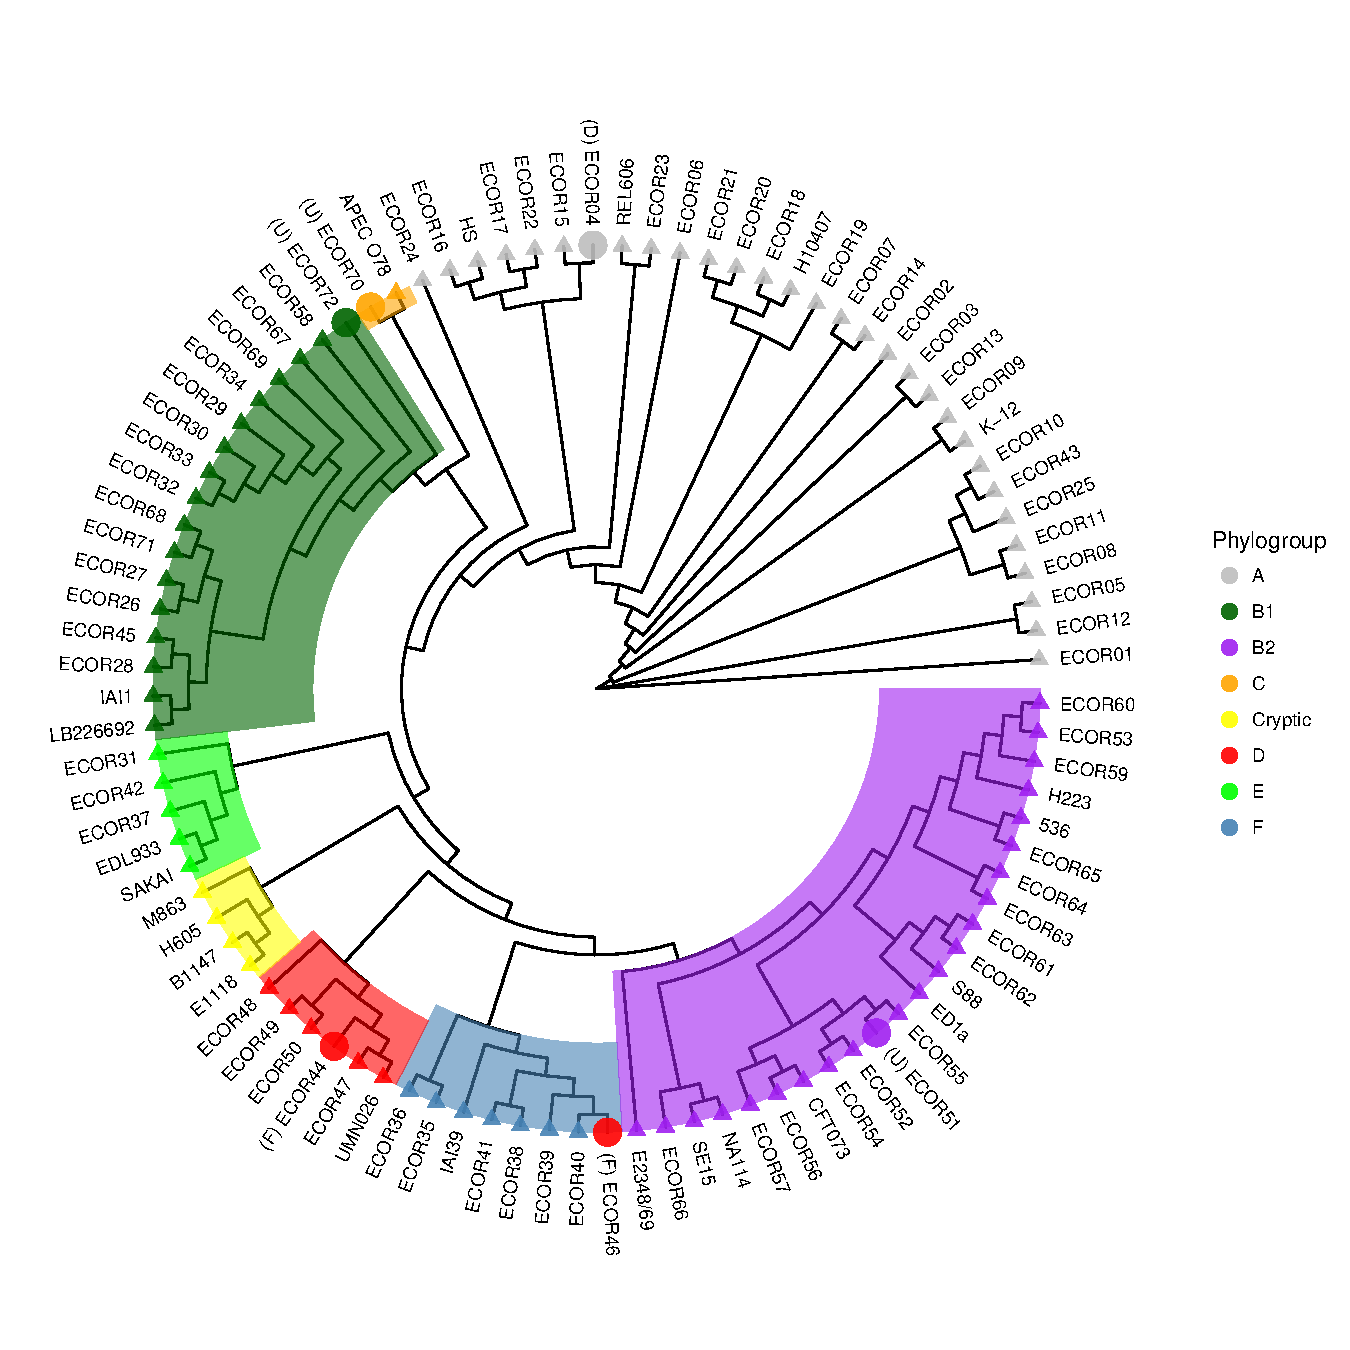
\includegraphics[width=.5\textwidth]{./analysis/cladogram.pdf}
  \caption{ Parsimony cladogram of strains from Clermont et al 2015. Tree was generated with kSNP3 (k=19). Enlarged circular tips show where EzClermont differed from reported phylogroup (EzClermont type show in brackets).}
  \label{fig:cladogram}
\end{figure}


Considering both the testing and validation datasets (114 strains), EzClermont has an accuracy of 94\%. Given the ease of use of the web app for simple queries, its incorporation into Enterobase, and the standalone speed of execution for larger batches, we hope that EzClermont will be of continued use to the scientific community.
